\chapter{Arhitektura i dizajn sustava}
		%\textbf{\textit{dio 1. revizije}}\\
		%\textit{ Potrebno je opisati stil arhitekture te identificirati: podsustave, preslikavanje na radnu platformu, spremišta podataka, mrežne protokole, globalni upravljački tok i sklopovsko-programske zahtjeve. Po točkama razraditi i popratiti odgovarajućim skicama:}
	%\begin{itemize}
	%	\item 	\textit{izbor arhitekture temeljem principa oblikovanja pokazanih na predavanjima (objasniti zašto ste baš odabrali takvu arhitekturu)}
	%	\item 	\textit{organizaciju sustava s najviše razine apstrakcije (npr. klijent-poslužitelj, baza podataka, datotečni sustav, grafičko sučelje)}
	%	\item 	\textit{organizaciju aplikacije (npr. slojevi frontend i backend, MVC arhitektura) }		
	%\end{itemize}
	Arhitektura se može podijeliti na tri podsustava:
	\begin{itemize}
		\item Web poslužitelj
		\item Web aplikacija
		\item Baza podataka
	\end{itemize}

	\underline{Web Klijent} je program koji omogućuje pregled web-stranica i multimedijskih sadržaja na istima s korisničkog računala. Izvorni kod internetskih stranica se interpretira na web pregledniku i prikazuje korisniku na pristupačan način i služi kao glavna pristupna točka aplikaciji s korisničke strane. Web preglednik je također zadužen za komunikaciju s web poslužiteljem putem zahtjeva.
	
	\underline{Web poslužitelj} je program koji obrađuje zahtjeve klijenata i šalje im odgovor, time omogućavajući klijentu komunikaciju s aplikacijom. Web poslužitelj je zadužen za obradu zahtjeva i slanje odgovora putem HTTP-a (engl.\textit{Hyper Text Transfer Protocol}), standardnog protokola za prijenos informacija na webu.
	
	\underline{Web aplikacija} je program kojemu je glavna svrha pružanje funkcionalnosti i usluga korisniku putem web preglednika u obliku HTML dokumenata. Web aplikacija je izgrađena na web poslužitelju i po potrebi komunicira s bazom podataka.
	
	\underline{Baza podataka} je sustav za pohranu podataka.

	Programski jezici u kojem je web aplikacija izrađena su Python zajedno s Flask web okvirom, te JavaScript zajedno s React web okvirom. Python je interpretirani, objektno orijentirani programski jezik visoke razine. Flask je mikro web okvir za Python koji omogućuje brzo i jednostavno kreiranje web aplikacija. JavaScript je interpretirani, dinamički programski jezik visoke razine. React je JavaScript biblioteka za izgradnju korisničkih sučelja. Odabrano razvojno okruženje je Microsoft Visual Studio Code.
	Arhitektura sustava temeljiti će se na MVC arhitekturi (engl. \textit{Model-View-Controller}). MVC dozvoljava nezavisan rad na različitim dijelovima aplikacije, što omogućava brži razvoj i održavanje cijelog sustava. Njezini dijelovi su:
	\begin{itemize}
		\item \textbf{Model} - Komponenta sustava odgovorna za pohranu i dohvat podataka. Predstavljena je dinamičkim strukturama podataka. Ima interakciju s Controller-om, od kojeg prima ulazne podatke te kojemu pruža podatke za prikaz.
		\item \textbf{View} - Komponenta sustava odgovorna za prikaz podataka korisniku. Može biti formatirana u obliku HTML dokumenata, kao JSON ili u drugom formatu. Ima interakciju s Controller-om, od kojeg prima podatke za prikaz.
		\item \textbf{Controller} - Komponenta sustava koja prima ulazne podatke i prosljeđuje ih Model-u ili View-u. Zadužena je za korisničke zahtjeve i odgovore te obavlja interakciju s ostalim komponentama sustava.
	\end{itemize}

	\begin{figure}[htbp]
		\centering
		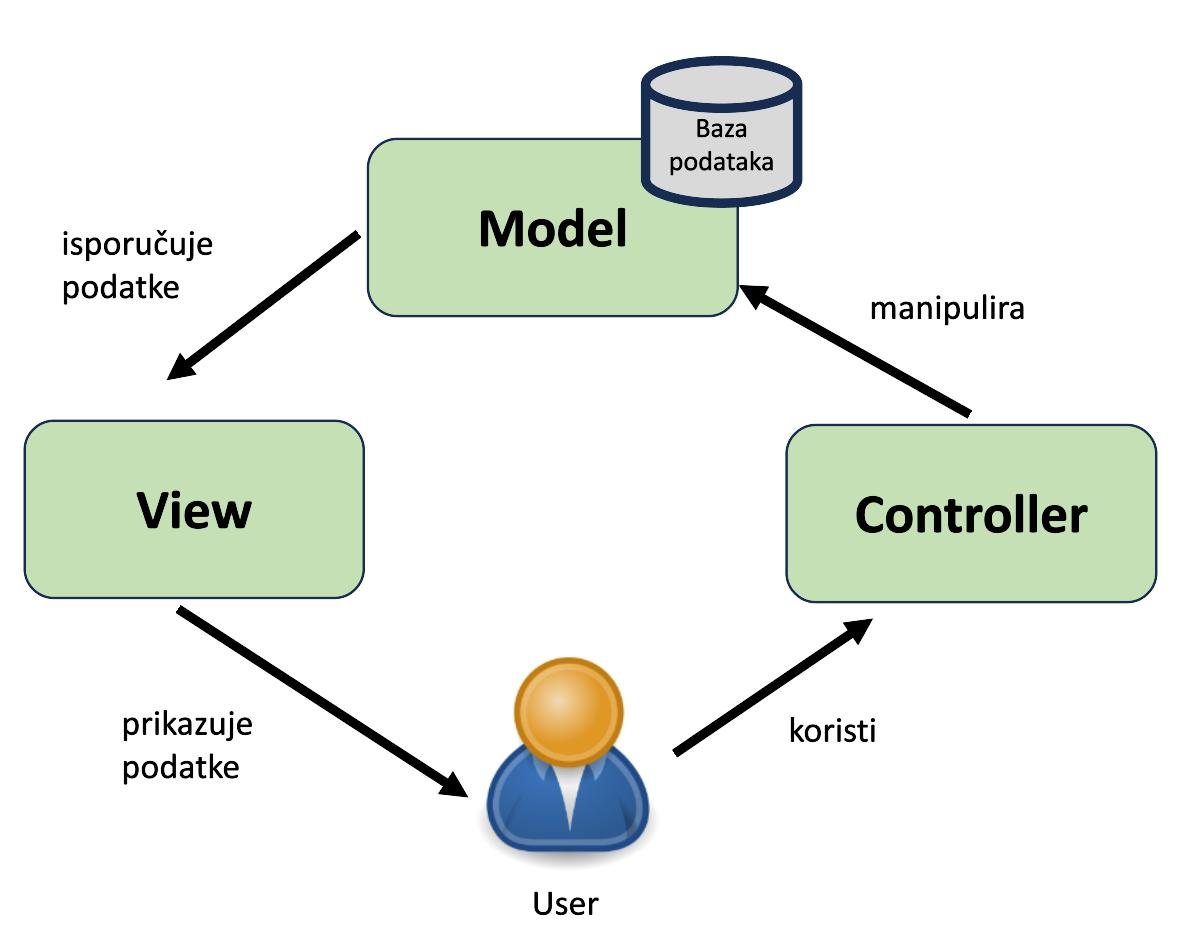
\includegraphics[width=1\textwidth]{slike/skica_mvc.jpg}
		\caption{Skica osnovne arhitekture sustava}
	\label{fig:my_image}
	\end{figure}

	%Osim navedenih dijelova arhitekture, dio poslovne logike se nalazi u sloju Service.
	

	\pagebreak
				
		\section{Baza podataka}
			
			%\textbf{\textit{dio 1. revizije}}\\
			
		%\textit{Potrebno je opisati koju vrstu i implementaciju baze podataka ste odabrali, glavne komponente od kojih se sastoji i slično.}
		
		\textrm{Za naš sustav koristit ćemo relacijsku bazu podataka čija je struktura pogodna za modeliranje stvarnog svijeta. Gradivna jedinka baze je relacija, odnosno tablica koja je definirana svojim imenom i skupom atributa. Zadaća baze podataka je brza i jednostavna pohrana, izmjena i dohvat podataka za obradu. Baza podataka naše aplikacije sastoji se od sljedećih entiteta:}
		
	\begin{packed_item}
		
		\item Račun
		\item Posjetitelj
		\item Organizator
		\item Pretplata
		\item Plaćanje
		\item Događanje
		\item Interes
		\item Recenzija
		\item Media-Događanje
		\item Država
		\item Vrsta Događanja
		\item Obavijest-Vrsta-Događanja
		\item Obavijest-Država
		\item Podatak
	\end{packed_item}
		
		
			\subsection{Opis tablica}
					

			%\textit{Svaku tablicu je potrebno opisati po zadanom predlošku. Lijevo se nalazi točno ime varijable u bazi podataka, u sredini se nalazi tip podataka, a desno se nalazi opis varijable. Svjetlozelenom bojom označite primarni ključ. Svjetlo plavom označite strani ključ}
			
			\textbf{Račun} \newline \textrm{ Ovaj entitet sadržava sve osnovne informacije o registriranom korisniku.
			Sadrži atribute: identifikator računa, korisničko ime, lozinka, e-mail, profilna slika, šifra država(ISO3), pripadna uloga.
			Ovaj entitet u vezi je \textit{One-to-One} s entitetima Posjetitelj i Organizator preko atributa accountId i u vezi \textit{Many-to-One} s entitetom Država preko atributa countryCode.}
			\begin{longtblr}[
				label=none,
				entry=none
				]{
					width = \textwidth,
					colspec={|X[6,l]|X[6, l]|X[20, l]|}, 
					rowhead = 1,
				} %definicija širine tablice, širine stupaca, poravnanje i broja redaka naslova tablice
				\hline \SetCell[c=3]{c}{\textbf{Account}}	 \\ \hline[3pt]
				\SetCell{LightGreen}accountId & INT	&  	jedinstveni identifikator računa  	\\ \hline
				username	& VARCHAR &  jedinstveni identifikator korisnika 	\\ \hline 
				eMail & VARCHAR & E-Mail korisnika  \\ \hline 
				passwordHash & VARCHAR	&  	raspršeno kriptirana lozinka korisnika	\\ \hline 
				profileImage & VARCHAR	&  	lokalna adresa na profilnu sliku korisnika	\\ \hline 
				\SetCell{LightBlue}countryCode & CHAR(3)	&  	jedinstveni id države kojoj račun pripada u formatu 3 slova (Država.countryCode) 	\\ \hline
				roleId & INT	&  	šifra uloge pridružene korisniku	\\ \hline 
			\end{longtblr}
			
			
			
			\textbf{Posjetitelj} \newline \textrm{ Ovaj entitet specijalizacija je entiteta Račun namijenjena za "obične" korisnike.
				Sadrži atribute: identifikator računa, ime i prezime.
				Ovaj entitet u vezi je \textit{One-to-One} s entitetom Račun i u
				vezi \textit{One-to-Many} s entitetima Interes, Recenzija, Opcija-Država i Opcija-Vrsta-Događanja preko atributa accountId.}
			\begin{longtblr}[
				label=none,
				entry=none
				]{
					width = \textwidth,
					colspec={|X[6,l]|X[6, l]|X[20, l]|}, 
					rowhead = 1,
				} %definicija širine tablice, širine stupaca, poravnanje i broja redaka naslova tablice
				\hline \SetCell[c=3]{c}{\textbf{Visitor}}	 \\ \hline[3pt]
				\SetCell{LightGreen}accountId & INT	&  	jedinstveni identifikator računa (Račun.accountId)  	\\ \hline
				firstName	& VARCHAR &  ime posjetitelja 	\\ \hline 
				lastName & VARCHAR & prezime posjetitelja  \\ \hline 
				
			\end{longtblr}
			
			\textbf{Organizator} \newline \textrm{ Ovaj entitet specijalizacija je entiteta Račun namijenjena za korisnike koji su organizatori.
				Sadrži atribute: identifikator računa, ime organizatora, vidljivost profila, poveznica na društvene mreže organizatora.
				Ovaj entitet u vezi je \textit{One-to-One} s entitetom Račun i u
				vezi \textit{One-to-Many} s entitetima s entitetima Plaćanje, Pretplata i Događanje preko atributa accountId.}
			\begin{longtblr}[
				label=none,
				entry=none
				]{
					width = \textwidth,
					colspec={|X[6,l]|X[6, l]|X[20, l]|}, 
					rowhead = 1,
				} %definicija širine tablice, širine stupaca, poravnanje i broja redaka naslova tablice
				\hline \SetCell[c=3]{c}{\textbf{Organizer}}	 \\ \hline[3pt]
				\SetCell{LightGreen}accountId & INT	&  	jedinstveni identifikator računa (Račun.accountId)   	\\ \hline

				organizerName	& VARCHAR &  naziv organizatora ili organizacije 	\\ \hline 
				hidden	& BOOLEAN &  zastavica koja govori o javnoj vidljivosti profila organizatora	\\ \hline 
				socials	& VARCHAR &  poveznica na društvene mreže organizatora.	\\ \hline 
									
			\end{longtblr}
			\pagebreak
			
			\textbf{Pretplata} \newline \textrm{ Ovaj entitet opisuje pretplatu koju je organizator nekad imao te koja može biti trenutno aktivna.
				Sadrži atribute: identifikator pretplate, datum početka pretplate, datum isteka pretplate, identifikator računa organizatora.
				Ovaj entitet u vezi je \textit{Many-to-One} s entitetom Organizator preko atributa accountId.}
			\begin{longtblr}[
				label=none,
				entry=none
				]{
					width = \textwidth,
					colspec={|X[6,l]|X[6, l]|X[20, l]|}, 
					rowhead = 1,
				} %definicija širine tablice, širine stupaca, poravnanje i broja redaka naslova tablice
				\hline \SetCell[c=3]{c}{\textbf{Subscription}}	 \\ \hline[3pt]
				\SetCell{LightGreen}subscriptionId & INT	&  	jedinstveni identifikator instance pretplate  	\\ \hline
				\SetCell{LightBlue}accountId & INT &  identifikator organizatora na kojeg se pretplata odnosi (Organizator.accountId) 	\\ \hline 
				startDate	& DATE &  datum početeka pretplate 	\\ \hline 
				expireDate	& DATE &  datum isteka pretplate 	\\ \hline 
			\end{longtblr}
			
			\textbf{Plaćanje} \newline \textrm{ Ovaj entitet opisuje plaćanje koje je organizator napravio prema našoj aplikaciji.
				Sadrži atribute: identifikator plaćanja, identifikator organizatora, datum plaćanja, iznos, metoda plaćanja.
				Ovaj entitet u vezi je \textit{Many-to-One} s entitetom Organizator preko atributa accountId.}
			\begin{longtblr}[
				label=none,
				entry=none
				]{
					width = \textwidth,
					colspec={|X[6,l]|X[6, l]|X[20, l]|}, 
					rowhead = 1,
				} %definicija širine tablice, širine stupaca, poravnanje i broja redaka naslova tablice
				\hline \SetCell[c=3]{c}{\textbf{Payment}}	 \\ \hline[3pt]
				\SetCell{LightGreen}paymentId & INT	&  	jedinstveni identifikator plaćanja 	\\ \hline
				\SetCell{LightBlue}accountId & INT &  identifikator organizatora na kojeg se plaćanje odnosi (Organizator.accountId) 	\\ \hline 
				date	& DATETIME &  datum i vrijeme plaćanja 	\\ \hline 
				amount	& FLOAT &  plaćen iznos 	\\ \hline 
				payment- Method	& VARCHAR &  način uplate 	\\ \hline 
			\end{longtblr}
			
			\pagebreak
			\textbf{Događanje} \newline \textrm{ Ovaj entitet opisuje događanje organizirano od strane organizatora.
				Sadrži atribute: identifikator događanja, identifikator organizatora, naziv, opis, državu, grad, lokaciju, datum i vrijeme, cijenu, naslovnu sliku događanja, 
				vrstu događanja, trajanje.
				Ovaj entitet u vezi je \textit{Many-to-One} s entitetima Organizator i Vrsta događanja preko atributa accountId i s entitetom Država preko atributa countryCode, 
				vezi \textit{One-to-Many} s entitetom Recenzija preko atributa eventId, vezi \textit{Many-to-Many} s entitetom Posjetitelj preko veze Interes i atributa eventId te u vezi \textit{One-to-Many} s entitetom Media-Događanje također preko atributa eventId.}
			\begin{longtblr}[
				label=none,
				entry=none
				]{
					width = \textwidth,
					colspec={|X[6,l]|X[6, l]|X[20, l]|}, 
					rowhead = 1,
				} %definicija širine tablice, širine stupaca, poravnanje i broja redaka naslova tablice
				\hline \SetCell[c=3]{c}{\textbf{Event}}	 \\ \hline[3pt]
				\SetCell{LightGreen}eventId & INT	&  	jedinstveni identifikator događanja 	\\ \hline
				\SetCell{LightBlue}accountId & INT &  identifikator organizatora koji organizira događanje (Organizator.accountId) 	\\ \hline 
				title	& VARCHAR &  naziv događanja 	\\ \hline 
				description	& VARCHAR &  opis događanja 	\\ \hline 
				price	& FLOAT &  cijena događanja 	\\ \hline 
				display- ImageSource	& VARCHAR &  lokalna adresa naslovne slike događanja 	\\ \hline 
				dateTime	& DATETIME &  vrijeme i datum događanja 	\\ \hline 
				countryCode	& CHAR(3) & šifra države u kojoj se događanje održava (Država.countryCode)	\\ \hline 
				city	& VARCHAR &  grad u kojem se događanje održava 	\\ \hline 
				location	& VARCHAR &  lokacija na kojoj se događanje održava	\\ \hline 
				price	& FLOAT &  cijena događanja 	\\ \hline
				duration & INTERVAL & trajanje događanja \\ \hline 
				\SetCell{LightBlue}eventType & INT &  identifikator vrste događanja (EventType.typeId)	\\ \hline
			\end{longtblr}
			
				\textbf{Interes} \newline \textrm{ Ovaj entitet predstavlja \textit{Many-to-Many} vezu interesa od strane Posjetitelja prema Događanju.
				Sadrži atribute: identifikator događanja, identifikator računa posjetitelja, stupanj zainteresiranosti.
				Ovaj entitet u vezi je \textit{Many-to-One} s entitetima Posjetitelj i Događanje preko atributa accountId i eventId.}
			\begin{longtblr}[
				label=none,
				entry=none
				]{
					width = \textwidth,
					colspec={|X[6,l]|X[6, l]|X[20, l]|}, 
					rowhead = 1,
				} %definicija širine tablice, širine stupaca, poravnanje i broja redaka naslova tablice
				\hline \SetCell[c=3]{c}{\textbf{Interest}}	 \\ \hline[3pt]
				\SetCell{LightGreen}eventId & INT	&  	indetifikator događanja na koje se interes odnosi (Događanje.eventId)	\\ \hline
				\SetCell{LightGreen}accountId & INT &  identifikator posjetitelja na kojeg se interes odnosi (Posjetitelj.accountId) 	\\ \hline 
				degreeOfInterest & INT &  stupanj interesa 	\\ \hline 
			\end{longtblr}
			
				\textbf{Recenzija} \newline \textrm{ Ovaj entitet modelira recenzije ostavljene od strane Posjetitelja za pojedina Događanja.
				Sadrži atribute: jedinstveni identifikator recenzije, identifikator događanja, identifikator računa posjetitelja, komentar, datum, vrijeme.
				Ovaj entitet u vezi je \textit{Many-to-One} s entitetima Događanje i Posjetitelj preko atributa eventId i accountId.}
			\begin{longtblr}[
				label=none,
				entry=none
				]{
					width = \textwidth,
					colspec={|X[6,l]|X[6, l]|X[20, l]|}, 
					rowhead = 1,
				} %definicija širine tablice, širine stupaca, poravnanje i broja redaka naslova tablice
				\hline \SetCell[c=3]{c}{\textbf{Review}}	 \\ \hline[3pt]
				\SetCell{LightGreen}reviewId & INT	&  	jedinstveni identifikator ostavljene recenzije	\\ \hline
				\SetCell{LightBlue}accountId & INT &  identifikator posjetitelja koji je ostavio recenziju (Posjetitelj.accountId) 	\\ \hline 
				\SetCell{LightBlue}eventId	& INT &  identifikator događanja na koje se recenzija odnosi (Događanje.eventId) 	\\ \hline 
				comment	& VARCHAR &  ostavljen komentar 	\\ \hline 
				dateTime	& DATETIME &  vrijeme i datum ostavljene recenzije 	\\ \hline 
			\end{longtblr}
			
			
			
				\textbf{Media-Događanje} \newline \textrm{ Ovaj entitet sprema lokalne adrese foto i video sadržaja koje pripada događanju.
				Sadrži atribute: jedinstveni identifikator recenzije, identifikator događanja, identifikator računa posjetitelja, komentar, datum, vrijeme.
				Ovaj entitet u vezi je \textit{Many-to-One} s entitetima Događanje i Posjetitelj preko atributa eventId i accountId.}
			\begin{longtblr}[
				label=none,
				entry=none
				]{
					width = \textwidth,
					colspec={|X[6,l]|X[6, l]|X[20, l]|}, 
					rowhead = 1,
				} %definicija širine tablice, širine stupaca, poravnanje i broja redaka naslova tablice
				\hline \SetCell[c=3]{c}{\textbf{EventMedia}}	 \\ \hline[3pt]
				\SetCell{LightGreen}mediaId & INT	&  	jedinstveni identifikator materijala	\\ \hline
				\SetCell{LightBlue}eventId	& INT &  identifikator događanja na koje se materijal odnosi (Događanje.eventId) 	\\ \hline 
				mediaType	& VARCHAR &  vrsta sadrđaja; slika ili video 	\\ \hline 
				mediaSource	& VARCHAR &  lokalna adresa sadržaja	\\ \hline 
			\end{longtblr}
			

			
			
				\textbf{Država} \newline \textrm{ Ovaj entitet modelira državu sa pripadnim šiframa i nazivom države.
				Sadrži atribute: identifikator države, sekundarni identifikator države, ime države.
				Ovaj entitet u vezi je \textit{One-to-Many} s entitetima Događanje i račun preko atributa countryCode.}
			\begin{longtblr}[
				label=none,
				entry=none
				]{
					width = \textwidth,
					colspec={|X[6,l]|X[6, l]|X[20, l]|}, 
					rowhead = 1,
				} %definicija širine tablice, širine stupaca, poravnanje i broja redaka naslova tablice
				\hline \SetCell[c=3]{c}{\textbf{Country}}	 \\ \hline[3pt]
				\SetCell{LightGreen}countryCode & CHAR(3)	&  	jedinstveni identifikator države sastavljen od 3 slova	\\ \hline
				code & CHAR(2)	&  	sekundarni jedinstveni identifikator države sastavljen od 2 slova	\\ \hline
				name & VARCHAR	&  	naziv države	\\ \hline
			\end{longtblr}

			\textbf{Vrsta Događanja} \newline \textrm{ Ovaj entitet modelira vrstu događanja koji je definiran za svako Događanje.
				Sadrži atribute: identifikator vrste, naziv vrste.
				Ovaj entitet u vezi je \textit{One-to-Many} s entitetima Događanje i Obavijest-Vrsta-Događanja preko atributa typeId.}
			\begin{longtblr}[
				label=none,
				entry=none
				]{
					width = \textwidth,
					colspec={|X[6,l]|X[6, l]|X[20, l]|}, 
					rowhead = 1,
				} %definicija širine tablice, širine stupaca, poravnanje i broja redaka naslova tablice
				\hline \SetCell[c=3]{c}{\textbf{EventType}}	 \\ \hline[3pt]
				\SetCell{LightGreen}typeId & INT	&  	jedinstveni identifikator vrste događanja	\\ \hline
				typeName & VARCHAR	&  	naziv vrste događanja	\\ \hline
			\end{longtblr}
			

			\textbf{Obavijest-Država} \newline \textrm{ Ovaj entitet sprema informaciju o tome koji korisnik ima preference za događanja u kojim državama.
			Sadrži atribute: identifikator posjetitelja, identifikator države.
			Ovaj entitet u vezi je \textit{Many-to-One} s entitetom Posjetitelj preko atributa accountId te s entitetom Država preko atributa countryCode.}
		\begin{longtblr}[
			label=none,
			entry=none
			]{
				width = \textwidth,
				colspec={|X[6,l]|X[6, l]|X[20, l]|}, 
				rowhead = 1,
			} %definicija širine tablice, širine stupaca, poravnanje i broja redaka naslova tablice
			\hline \SetCell[c=3]{c}{\textbf{NotificationCountry}}	 \\ \hline[3pt]
			\SetCell{LightGreen}accountId & INT	&  	jedinstveni identifikator posjetitelja (Posjetitelj.accountId)	\\ \hline
			\SetCell{LightGreen}countryCode & CHAR(3)	&  identifikator države (Country.countryCode). (Primarni ključ je uređeni par accountId, countryCode)	\\ \hline
		\end{longtblr}

			\textbf{Obavijest-Vrsta-Događanja} \newline \textrm{ Ovaj entitet sprema informaciju o tome koji korisnik ima preference za vrstu događanja.
			Sadrži atribute: identifikator posjetitelja, identifikator vrste događanja.
			Ovaj entitet u vezi je \textit{Many-to-One} s entitetom Posjetitelj preko atributa accountId te s entitetom Vrsta Događanja preko atributa eventType.}
		\begin{longtblr}[
			label=none,
			entry=none
			]{
				width = \textwidth,
				colspec={|X[6,l]|X[6, l]|X[20, l]|}, 
				rowhead = 1,
			} %definicija širine tablice, širine stupaca, poravnanje i broja redaka naslova tablice
			\hline \SetCell[c=3]{c}{\textbf{NotificationEventType}}	 \\ \hline[3pt]
			\SetCell{LightGreen}accountId & INT	&  	jedinstveni identifikator posjetitelja (Posjetitelj.accountId)	\\ \hline
			\SetCell{LightGreen}typeId & INT	&  identifikator vrste događanja (EventType.typeId). (Primarni ključ je uređeni par accountId, eventType)	\\ \hline
		\end{longtblr}


			\textbf{Podaci} \newline \textrm{ Ovaj entitet zadužen je spremati različite podatke potrebne za funkcioniranje i prezistenciju poslužiteljske strane.
					Sadrži atribute: naziv varijable, vrijednost varijable u string formatu.
					Ovaj entitet nije povezan s niti jednim drugim entitetom. Služi kao "look-up" tablica.}
		\begin{longtblr}[
			label=none,
			entry=none
			]{
				width = \textwidth,
				colspec={|X[6,l]|X[6, l]|X[20, l]|}, 
				rowhead = 1,
			} %definicija širine tablice, širine stupaca, poravnanje i broja redaka naslova tablice
			\hline \SetCell[c=3]{c}{\textbf{Data}}	 \\ \hline[3pt]
			\SetCell{LightGreen}entryName & VARCHAR	&  	naziv varijable	\\ \hline
			value & VARCHAR	&  vrijednost varijable u string formatu	\\ \hline
		\end{longtblr}



			\pagebreak
		\subsection{Dijagram baze podataka}
				%\textit{ U ovom potpoglavlju potrebno je umetnuti dijagram baze podataka. Primarni i strani ključevi moraju biti označeni, a tablice povezane. Bazu podataka je potrebno normalizirati. Podsjetite se kolegija "Baze podataka".}
				
				\begin{figure}[htbp]
					\centering
					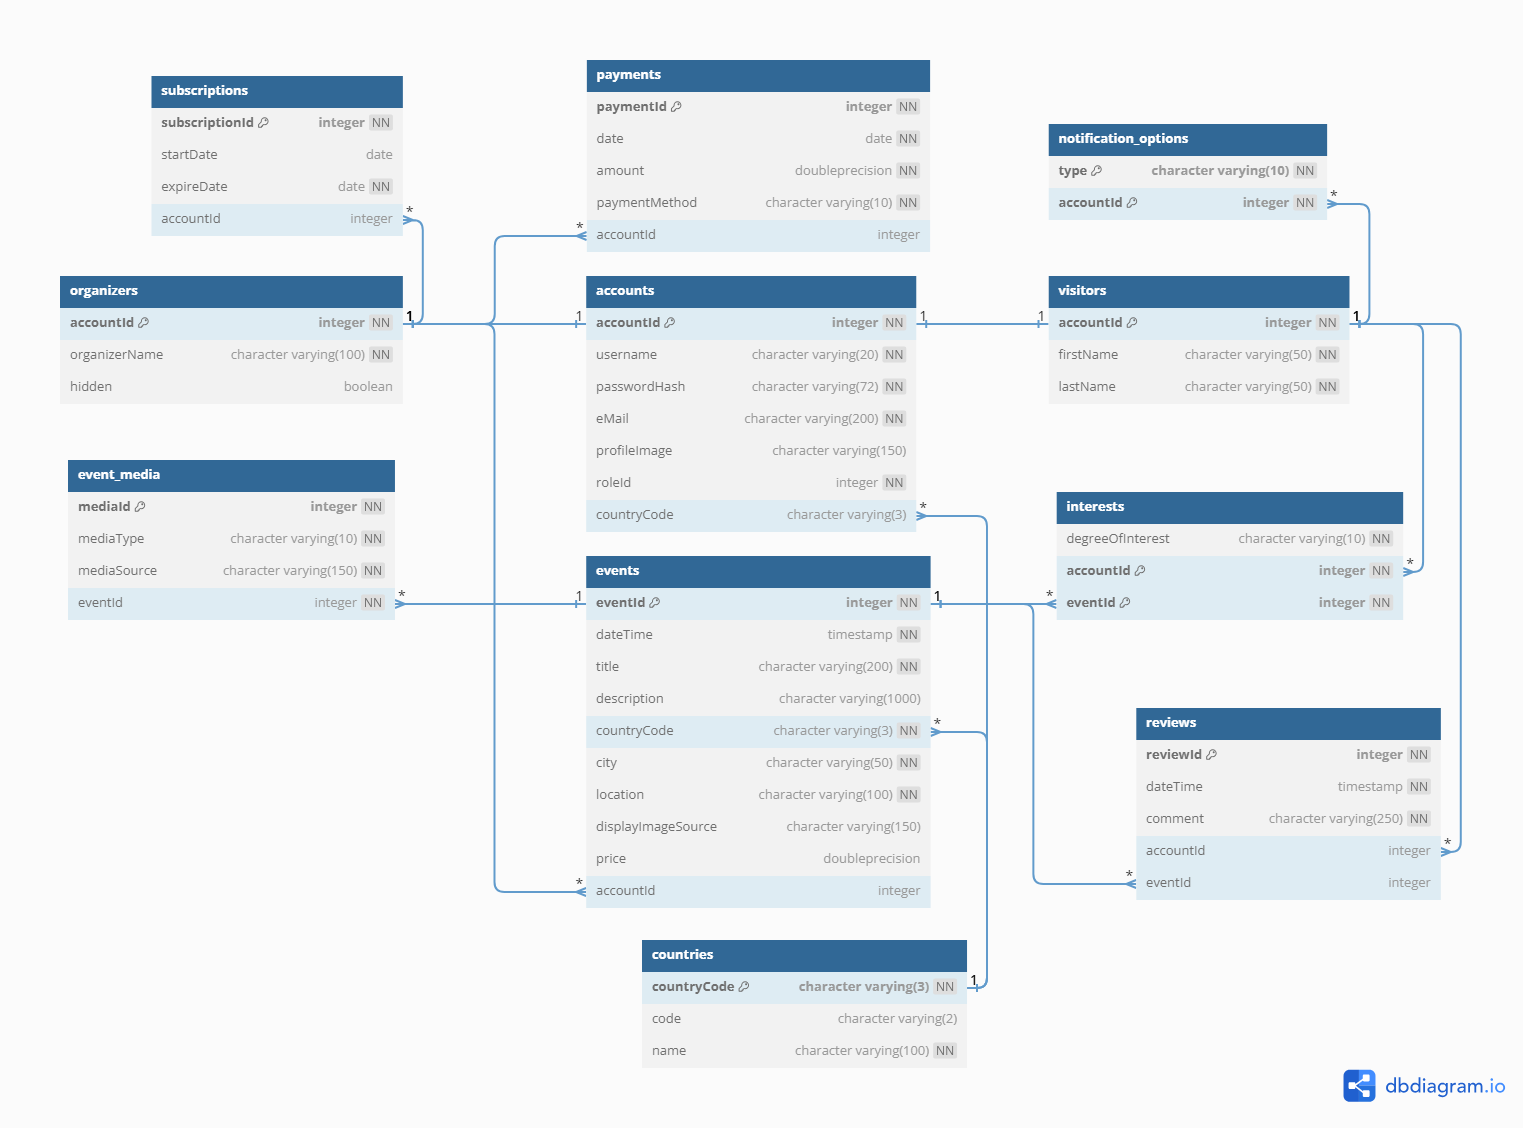
\includegraphics[width=1\textwidth]{dijagrami/relacijski_dijagram.png}
					\caption{Relacijski dijagram baze podataka}
					\label{fig:my_image}
				\end{figure}
				
				
	
			\eject
			
		\newpage	
		\section{Dijagram razreda}
		
			%\textit{Potrebno je priložiti dijagram razreda s pripadajućim opisom. Zbog preglednosti je moguće dijagram razlomiti na više njih, ali moraju biti grupirani prema sličnim razinama apstrakcije i srodnim funkcionalnostima.}\\
			%\textbf{\textit{dio 1. revizije}}\\
			%\textit{Prilikom prve predaje projekta, potrebno je priložiti potpuno razrađen dijagram razreda vezan uz \textbf{generičku funkcionalnost} sustava. Ostale funkcionalnosti trebaju biti idejno razrađene u dijagramu sa sljedećim komponentama: nazivi razreda, nazivi metoda i vrste pristupa metodama (npr. javni, zaštićeni), nazivi atributa razreda, veze i odnosi između razreda.}\\
			%\textbf{\textit{dio 2. revizije}}\\			
			%\textit{Prilikom druge predaje projekta dijagram razreda i opisi moraju odgovarati stvarnom stanju implementacije}
			
			\textit{}

			Na slikama 4.2, 4.3 i 4.4 prikazani su dijagrami razreda za podsustave u backend dijelu arhitekture. Na slici 4.3. prikazani su razredi koji nasljeđuju Controller razred. Metode tih razreda koriste Model razrede za dohvat i spremanje podataka. Metode u razredima Controller vraćaju JSON datoteke u obliku HTML status koda i podatkovnog dijela. Na slici 4.4 prikazani su Data Transfer objekti. Na slici 4.5. prikazani su razredi koji nasljeđuju Model razred i predstavljaju (modeliraju) entitete baze podataka.
			
			Zbog lakše organizacije i vidljivosti dijagrama razreda, razredi su podijeljeni u više dijagrama. Razredi su grupirani prema sličnim razinama apstrakcije i srodnim funkcionalnostima u arhitekturi MVC.
			
			\begin{figure}[htbp]
				\centering
				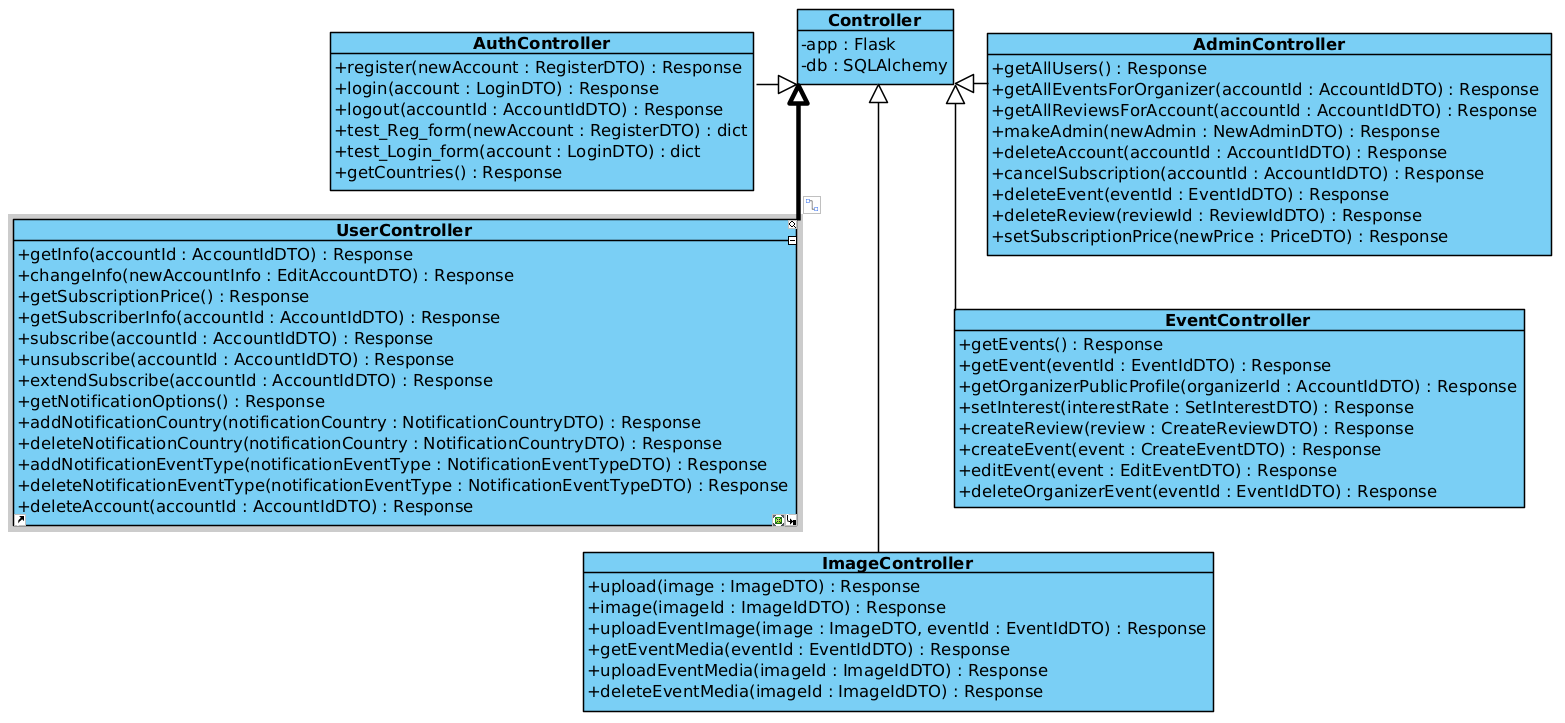
\includegraphics[width=1\textwidth]{dijagrami/dijagram_mvc_controllers.png}
				\caption{Dijagram klasa, dio Controllers}
			\label{fig:my_image}
			\end{figure}

			\newpage

			\begin{figure}[htbp]
				\centering
				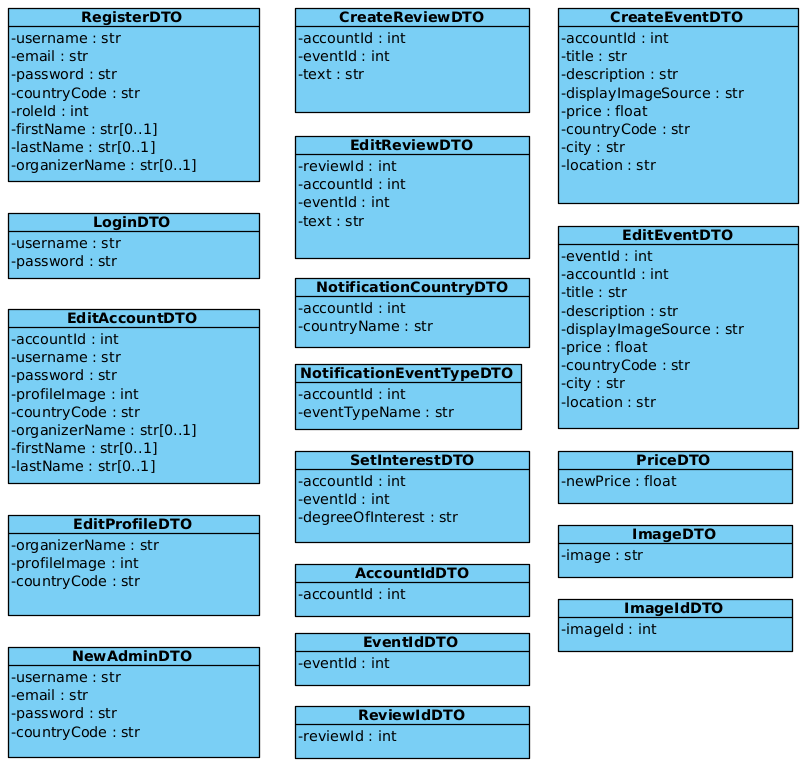
\includegraphics[width=1\textwidth]{dijagrami/dijagram_mvc_dto.png}
				\caption{Dijagram klasa, dio DTO}
			\label{fig:my_image}
			\end{figure}

			\newpage

			\begin{figure}[htbp]
				\centering
				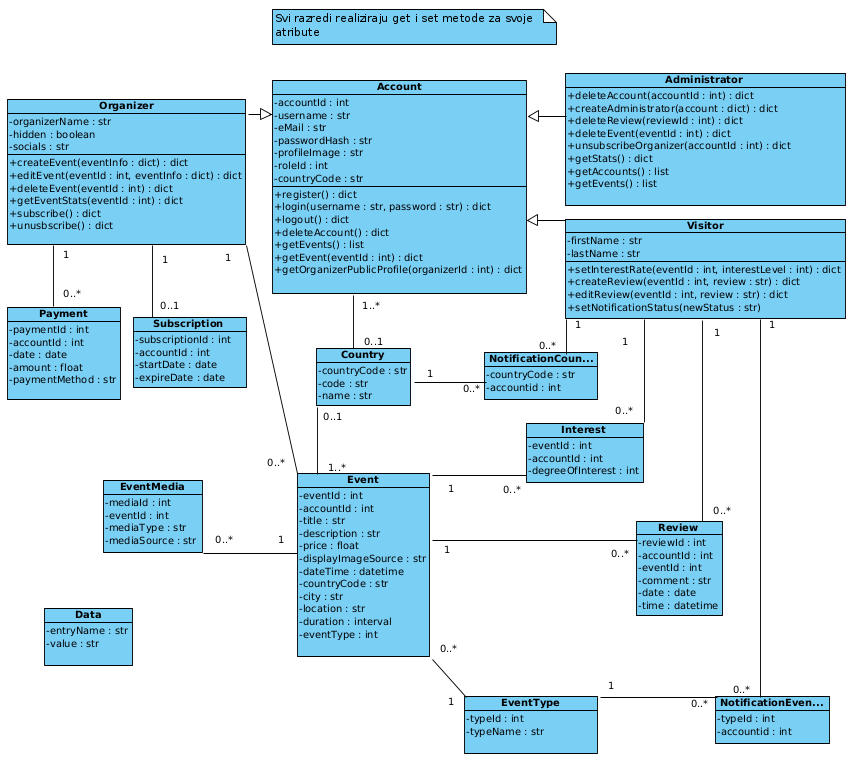
\includegraphics[width=1\textwidth]{dijagrami/dijagram_mvc_models.png}
				\caption{Dijagram klasa, dio Models}
			\label{fig:my_image}
			\end{figure}


			\eject
		
		\newpage
		\section{Dijagram stanja}
			
			% \textbf{\textit{dio 2. revizije}}\\
			
			% \textit{Potrebno je priložiti dijagram stanja i opisati ga. Dovoljan je jedan dijagram stanja koji prikazuje \textbf{značajan dio funkcionalnosti} sustava. Na primjer, stanja korisničkog sučelja i tijek korištenja neke ključne funkcionalnosti jesu značajan dio sustava, a registracija i prijava nisu. }
			Dijagram stanja opisuje dinamičko ponašanje dijela sustava.
			Prikazuje stanja objekta te prijelaze temeljene na događajima.
			Na slici 4.5 prikazan je dijagram stanja za registriranog organizatora.
			Nakon prijave, organizatoru se prikazuje početna stranica na kojoj se nalaze svi događaji.
			Klikom na "See More" gumb na pojedinom događaju, organizatoru se prikazuje kartica događaja.
			Ako je organizator vlasnik događaja, ima mogućnost uređivanja događaja.
			Na stranici postoji bočna traka koja služi za navigaciju kroz aplikaciju.
			Klikom na "Profile" organizatoru se prikazuje njegov javni profil.
			Klikom na "Account" prikazuje se stranica za pregled i uređivanje osobnih podataka te profilne slike.
			Klikom na "ConnectiNET Premium" prikazuje se stranica za upravljanje pretplatom.
			Odabirom "Create Event" organizatoru se prikazuje stranica za stvaranje novog događaja.


			\begin{figure}[htbp]
				\centering
				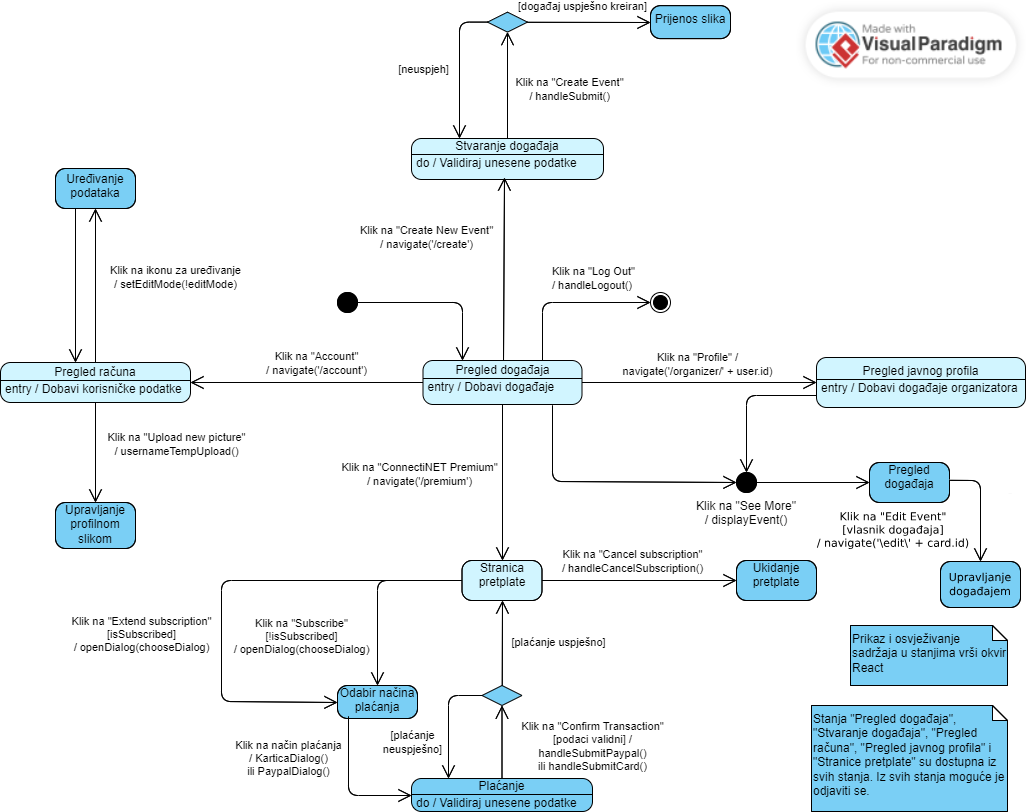
\includegraphics[width=1\textwidth]{dijagrami/dijagram_stanja.png}
				\caption{Dijagram stanja}
			\end{figure}
			
			\eject 
		
		\section{Dijagram aktivnosti}
			
			%\textbf{\textit{dio 2. revizije}}\\
			
			 %\textit{Potrebno je priložiti dijagram aktivnosti s pripadajućim opisom. Dijagram aktivnosti treba prikazivati značajan dio sustava.}\\
			 Na dijagramu aktivnosti prikazan je proces ostavljanja recenzije od strane korisnika. Korisnik se najprije prijavi u sustav ako je već jednom uspješno završio proces registracije. Nakon toga odabirom opcije pregleda događaja dolazi do popisa svih trenutno evidentiranih događaja u bazi podataka nad kojim odabirom neke od funkcija za kontrolu pregleda (sortiranje, filtriranje, traženje ključne riječi) reducira izbor prema vlastitim željama. Kada pronađe i odabere željeni događaj otvara mu se prikaz s dodatnim informacijama o dotičnom događaju. Ako je događaj završio unazad 48 sati, Korisnik odabirom funkcije za ostavljenje recenzija popunjava obrazac za ostavljanje recenzije. Ispravnim popunjavanjem obrasca, recenzija se pohranjuje u bazi podataka.  
			 \begin{figure}[htbp]
				\centering
				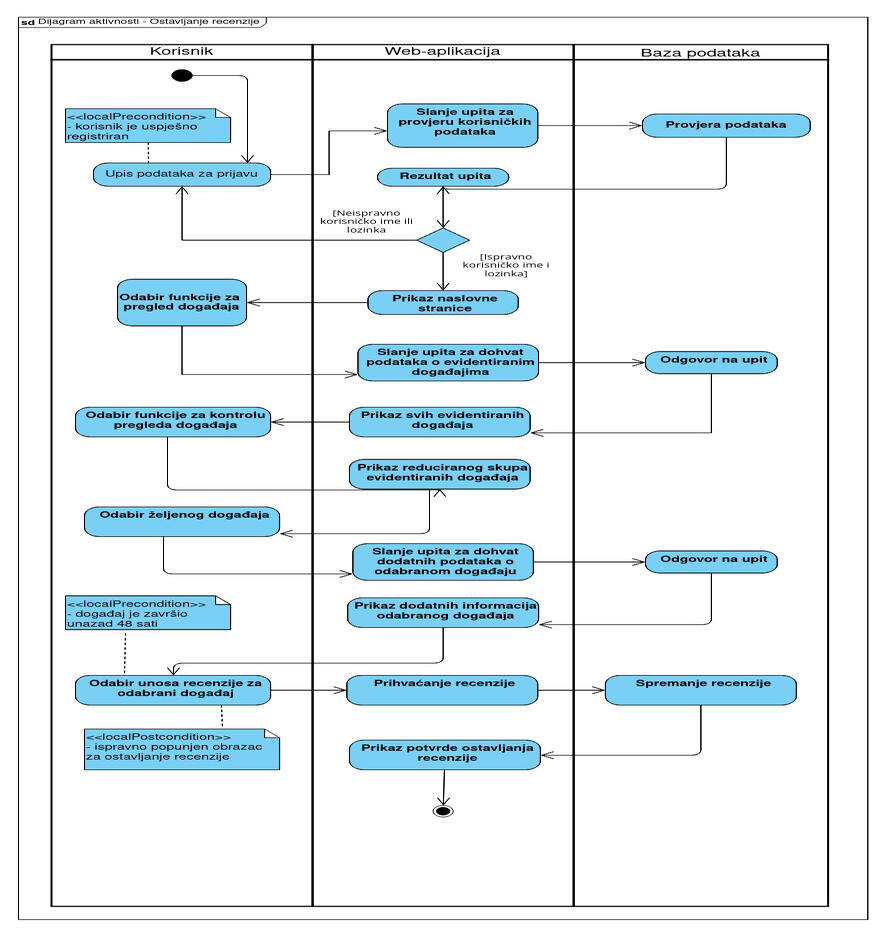
\includegraphics[width=1\textwidth]{dijagrami/diagram_aktivnosti_finally.jpeg} %height=0.7\textheight
				\caption{Dijagram aktivnosti}
			\label{fig:my_image}
			\end{figure}

			\eject
		\section{Dijagram komponenti}
		
			%\textbf{\textit{dio 2. revizije}}\\
		
			 %\textit{Potrebno je priložiti dijagram komponenti s pripadajućim opisom. Dijagram komponenti treba prikazivati strukturu cijele aplikacije.}
			 Sustavu se pristupa preko dva različita sučelja. Preko sučelja za dohvat HTML, CSS, JS i JSX datoteka poslužuju se datoteke koje pripadaju frontend dijelu aplikacije. Router je komponenta koja na upit s url-a određuje koja datoteka će se poslužiti na sučelje. Frontend dio se sastoji od većeg broja JavaScript datoteka koje su raspoređene u logičke cjeline views, ui i context. Views datoteke definiraju osnovnu strukturu stranice koja će se prikazati korisniku. Ui datoteke predstavljaju komponente koje dopunjuju strukturu stranice. Context sadrži kontekste koji olakšavaju dijeljenje podataka između React komponenata. ProtectedComponent.jsx datoteka je React komponenta koja služi kao zaštitni omotač za druge komponente. Koristi se za provjeru je li korisnik prijavljen i ima li odgovarajuće ovlasti za pristup određenim dijelovima aplikacije. Ako korisnik nije prijavljen ili nema odgovarajuće ovlasti, komponenta preusmjerava korisnika na stranicu za prijavu ili na drugu stranicu. Sve JavaScript datoteke ovise o React biblioteci iz koje dohvaćaju gotove komponente kao što su gumbi, forme i slično. Preko sučelja za dohvat JSON podataka pristupa se REST API komponenti. REST API poslužuje podatke koji pripadaju backend dijelu aplikacije. SQLAlchemy je zadužen za dohvaćanje tablica iz baze podataka pomoću SQL upita. Podaci koji su pristigli iz baze se šalju dalje MVC arhitekturi u obliku jednostavnih Python klasa ili tuple-ova koji se kasnijom obradom pretvaraju u JSON objekte. Util.py implementira sučelje koje se koristi za provjeru prava pristupa određenim podacima i rutama. React-view komponenta preko oba sučelja komunicira s ConnectiNET aplikacijom te ovisno o korisnikovim akcijama osvježava prikaz i dohvaća nove podatke ili datoteke. Oba sučelja ovise o komponenti DataController.js koja preuzetim zahtjevima s korisničkog sučelja dodaje potrebne parametre i šalje zahtjev na poslužitelj. Kada poslužitelj vrati odgovor, DataController.js obrađuje taj odgovor i prosljeđuje ga natrag korisničkom sučelju.
			 \begin{figure}[htbp]
				\centering
				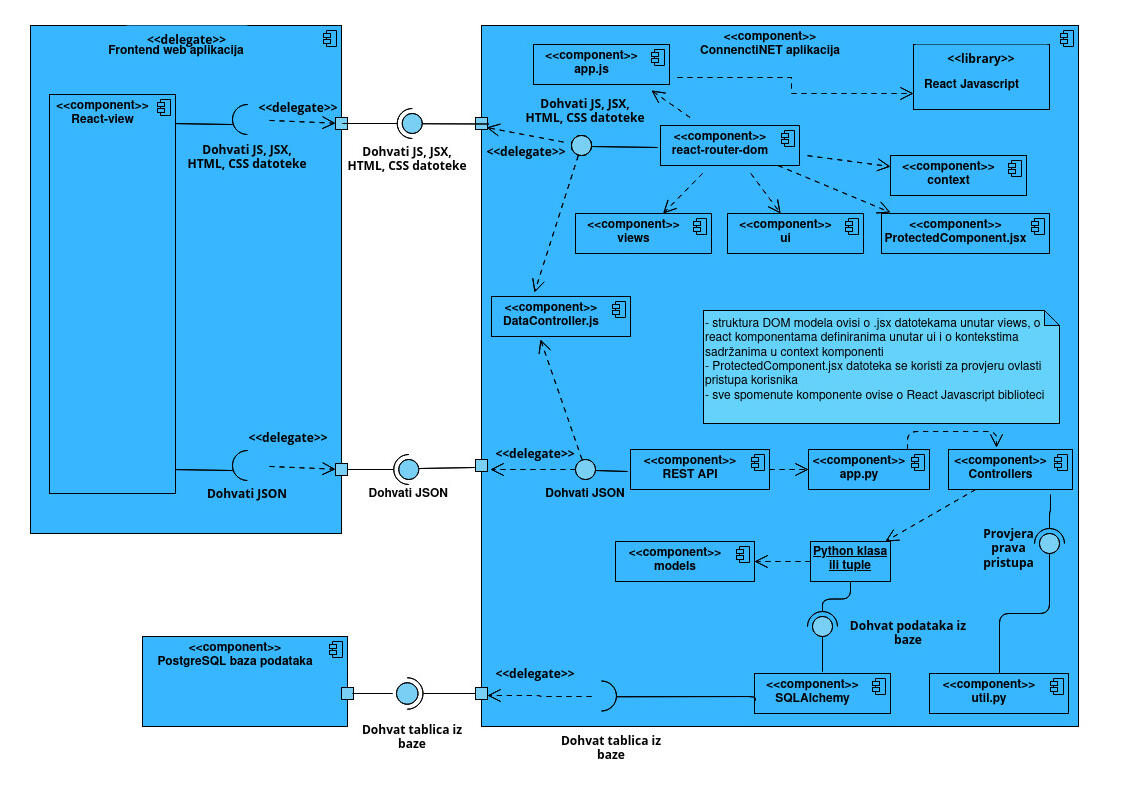
\includegraphics[width=1\textwidth]{dijagrami/component_diagram_finally.jpeg}
				\caption{Dijagram komponenti}
			\label{fig:my_image}
			\end{figure}